% Options for packages loaded elsewhere
\PassOptionsToPackage{unicode}{hyperref}
\PassOptionsToPackage{hyphens}{url}
%
\documentclass[
]{article}
\usepackage{amsmath,amssymb}
\usepackage{iftex}
\ifPDFTeX
  \usepackage[T1]{fontenc}
  \usepackage[utf8]{inputenc}
  \usepackage{textcomp} % provide euro and other symbols
\else % if luatex or xetex
  \usepackage{unicode-math} % this also loads fontspec
  \defaultfontfeatures{Scale=MatchLowercase}
  \defaultfontfeatures[\rmfamily]{Ligatures=TeX,Scale=1}
\fi
\usepackage{lmodern}
\ifPDFTeX\else
  % xetex/luatex font selection
\fi
% Use upquote if available, for straight quotes in verbatim environments
\IfFileExists{upquote.sty}{\usepackage{upquote}}{}
\IfFileExists{microtype.sty}{% use microtype if available
  \usepackage[]{microtype}
  \UseMicrotypeSet[protrusion]{basicmath} % disable protrusion for tt fonts
}{}
\makeatletter
\@ifundefined{KOMAClassName}{% if non-KOMA class
  \IfFileExists{parskip.sty}{%
    \usepackage{parskip}
  }{% else
    \setlength{\parindent}{0pt}
    \setlength{\parskip}{6pt plus 2pt minus 1pt}}
}{% if KOMA class
  \KOMAoptions{parskip=half}}
\makeatother
\usepackage{xcolor}
\usepackage[margin=1in]{geometry}
\usepackage{graphicx}
\makeatletter
\def\maxwidth{\ifdim\Gin@nat@width>\linewidth\linewidth\else\Gin@nat@width\fi}
\def\maxheight{\ifdim\Gin@nat@height>\textheight\textheight\else\Gin@nat@height\fi}
\makeatother
% Scale images if necessary, so that they will not overflow the page
% margins by default, and it is still possible to overwrite the defaults
% using explicit options in \includegraphics[width, height, ...]{}
\setkeys{Gin}{width=\maxwidth,height=\maxheight,keepaspectratio}
% Set default figure placement to htbp
\makeatletter
\def\fps@figure{htbp}
\makeatother
\setlength{\emergencystretch}{3em} % prevent overfull lines
\providecommand{\tightlist}{%
  \setlength{\itemsep}{0pt}\setlength{\parskip}{0pt}}
\setcounter{secnumdepth}{-\maxdimen} % remove section numbering
\usepackage{multicol}
\usepackage{natbib}
\usepackage{graphicx}
\usepackage{caption}
\usepackage{subcaption}
\usepackage{changepage}
\ifLuaTeX
  \usepackage{selnolig}  % disable illegal ligatures
\fi
\usepackage{bookmark}
\IfFileExists{xurl.sty}{\usepackage{xurl}}{} % add URL line breaks if available
\urlstyle{same}
\hypersetup{
  pdftitle={Linux Authentication and PAM},
  pdfauthor={Henry Roeth},
  hidelinks,
  pdfcreator={LaTeX via pandoc}}

\title{Linux Authentication and PAM}
\usepackage{etoolbox}
\makeatletter
\providecommand{\subtitle}[1]{% add subtitle to \maketitle
  \apptocmd{\@title}{\par {\large #1 \par}}{}{}
}
\makeatother
\subtitle{Face Recognition}
\author{Henry Roeth}
\date{2024-02-16}

\begin{document}
\maketitle
\begin{abstract}
In computer security, authentication is the process of confirming
someone is who they claim to be when attempting to access any kind of
computer system through the confirmation of something they have,
something they know, or something they are. It is important to always
maintain and improve the integrity of computer systems' authentication
schemes as new security threats arise. The Linux kernel invokes the
standard Unix authentication process across the majority of its
applications. However, as new forms of authentication are developed, it
is inefficient to individually reconfigure applications such that the
desired authentication scheme is incorporated. The PAM (Pluggable
Authentication Module) mechanism in Linux integrates various low-level
authentication schemes into a high-level API, allowing programs that
require some form of authentication to be developed independently from
the desired authentication scheme. This integrated research aims to
demonstrate the function and importance of PAM in Linux authentication
with the invocation of a face recognition PAM security module. Real-time
face detection and recognition is performed using the Haar Cascade
Classifier and the LBPH (Local Binary Patterns Histograms) feature-based
face recognition method.
\end{abstract}

\begin{multicols}{2}

\section{Introduction}
The Linux kernel invokes the standard Unix authentication process across most of its applications (e.g., common-auth, sshd, su, and sudo). When developers are creating and updating applications, it would prove quite inefficient to individually reconfigure application logic such that it aligns with the newly desired authentication scheme. This would mean restructuring code and requiring other dependencies. With this in mind, developers need a way to invoke authentication schemes independently from applications, allowing for a more modular approach. This enables programs to run separately. Much like it's father kernel (Unix) the Linux kernel invokes these modular authentication schemes via the PAM (Pluggable Authentication Module) mechanism. One might think of this as a multitool. Just as a multitool can have different tools for various purposes like cutting, screwing, or opening, PAM provides different authentication methods for Linux. Depending on what you need to authenticate—be it through passwords, biometrics, or other means—you can plug in the appropriate tool/module into PAM to handle the authentication process effectively. This integrated research aims to display this function with the creation of a modular authentication scheme—face recognition.

\section{The Linux Kernel}
The Linux kernel, at the heart of the Linux operating system, is a marvel of open-source collaboration and engineering excellence. Designed with modularity, efficiency, and stability in mind, it serves as the foundation upon which diverse computing systems are built (\cite{tanenbaum2012linux}). At its core, the Linux kernel follows a monolithic design, where essential functionalities like process management, memory management, device drivers, file system support, and networking protocols are tightly integrated into a single, cohesive entity. However, this monolithic structure doesn't imply rigidity; rather, it offers flexibility through loadable kernel modules that can be dynamically loaded and unloaded, allowing for on-demand expansion of kernel functionality without requiring a full kernel recompilation. The organization of the Linux kernel is characterized by its hierarchical structure and clear separation of concerns. The source code is divided into various subsystems, each responsible for a specific aspect of system operation. This modular approach not only simplifies development and maintenance but also enables developers to focus on specific areas without being overwhelmed by the entire codebase. Moreover, the Linux kernel's development process is highly collaborative, with thousands of contributors from around the world continuously refining and enhancing its codebase. This distributed development model, facilitated by tools like Git and mailing lists, fosters innovation and ensures that the kernel evolves in response to emerging technologies and changing user needs while maintaining backward compatibility. Additionally, the Linux kernel adheres to the principles of openness and transparency, with its source code being freely available for inspection, modification, and redistribution under the terms of the GNU General Public License (GPL). This openness not only promotes community involvement but also facilitates portability, enabling the kernel to run on a wide range of hardware architectures, from embedded devices to supercomputers. Furthermore, the Linux kernel's robustness and scalability have made it the preferred choice for powering critical infrastructure, including servers, cloud platforms, and mobile devices, cementing its position as one of the most influential and widely used pieces of software in the computing world.

\section{Overview of Linux Authentication}
Linux authentication involves several components. Centrally are the /etc/passwd and /etc/shadow files. In `/etc/passwd`, user account information such as usernames, user IDs, group IDs, and home directories are stored. The tangible passwords are more securely stored in `/etc/shadow`. It is here where there are hashed passwords and other security-related information. Each line in `/etc/shadow` represents a user account and includes uniquely populated fields like usernames, encrypted passwords, password aging and expiration details, and account lockout information. When any user attempts to login to the machine, the system hashes the entered password using the same algorithm as the one stored in /etc/shadow. If the hashed passwords match, access is granted to the user. More specifically, hashing involves the conversion of a password into a fixed-length string of characters using a cryptographic hash function. This process is irreversible, meaning the original password cannot be easily derived from the hash. Another additional measure of security that is implemented in the hashing process is salting. Salting is where a random value (a salt) is added to the password before hashing. This prevents attackers from using precomputed hash tables, also known as rainbow tables, to crack passwords. These unique fields in the /etc/shadow file are separated by colons, with each field serving a specific purpose. These fields may typically include the username, the hashed password, the last password date, the minimum and maximum password age, the password warning period, the password inactivity period, the account expiration date, and the account expiration date warning. To summarize, the integrity of the Linux authentication process relies on secure data storage of hashed passwords, salting for additional security, and an automated management system of user account information. As this relates to PAM, the invoked module (found in the directory /lib/*/security) is the primary logic to which the input password is hashed and compared to the corresponding hash in the /etc/shadow file; it is then followed by either a success or failure being return to the PAM mechanism.

\section{Hashing}
Hashing plays a pivotal role in Linux authentication mechanisms, safeguarding user credentials stored on the system. In Linux, password hashes are typically generated using cryptographic hash functions such as SHA-256 or SHA-512. When a user sets or updates their password, the system computes the hash of the password and stores it in the system's password file (`/etc/shadow`). When a user attempts to log in, the system hashes the provided password using the same algorithm and compares it with the stored hash in the password file. If the hashes match, access is granted. Otherwise, access is denied. This process ensures that even if an attacker gains access to the password file, obtaining the original passwords is exceedingly difficult due to the one-way nature of cryptographic hashing. According to \cite{doe2020survey}, hash functions are crucial for data integrity verification in authentication systems, emphasizing properties like collision resistance, which are essential for robust security implementations.

\section{Salts}
Salts are key in enhancing the security of password storage in Linux. When a user sets or changes their password, a random salt is generated and combined with the password before hashing. This salt is then stored alongside the hashed password in the system's password file. The purpose of the salt is to prevent attackers from using precomputed hash tables, such as rainbow tables, to quickly determine the original password from its hash. By adding a unique salt to each password before hashing, even if two users have the same password, their hashed values will be different due to the different salts used. Consequently, rainbow table attacks become impractical, as attackers would need to generate a new table for each unique salt value. This significantly increases the complexity and time required for password cracking attempts. Salting effectively mitigates various password-based attacks, thereby strengthening the overall security of the Linux authentication system (\cite{smith2021importance}).

\end{multicols}

\begin{figure}[htbp]
  \centering
  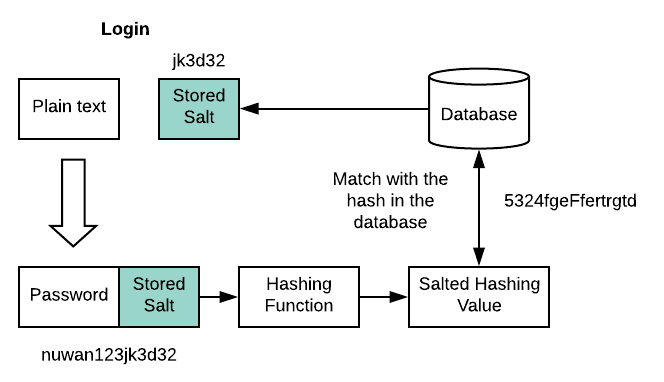
\includegraphics[width=0.4\linewidth]{images/salting.png}
  \caption{Linux Salting Process}
\end{figure}

\begin{multicols}{2}

\section{PAM Configuration}
Pluggable Authentication Modules (PAM) constitute a critical component of Linux systems, providing a flexible framework for authentication management. PAM enables system administrators to configure authentication policies independently of the applications requiring authentication, thus promoting modularity and security. Central to PAM's functionality are its configuration files located in `/etc/pam.d/`, which define the authentication rules for specific services or applications. These configuration files specify the modules to be invoked during authentication, such as password verification, account validation, and session management. Each module performs a specific authentication task, allowing administrators to tailor authentication mechanisms according to their security requirements. PAM modules can employ various authentication methods, including traditional password-based authentication, token-based authentication, biometric authentication, and multi-factor authentication. Additionally, PAM's modular design allows for the inclusion of custom authentication modules located in `/lib/*/security`, enabling further customization and integration with external authentication services, such as LDAP or Kerberos. This flexibility, coupled with PAM's extensibility, makes it a cornerstone of Linux security, facilitating robust authentication mechanisms that can adapt to diverse system architectures and security policies (\cite{jones2022importance}). 

\end{multicols}

\begin{figure}[htbp]
  \centering
  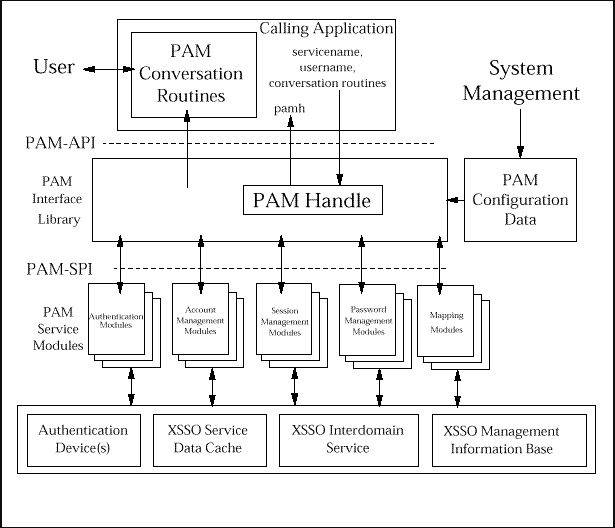
\includegraphics[width=0.4\linewidth]{images/pam_configuration.png}
  \caption{PAM System Framework}
\end{figure}

\begin{multicols}{2}

\section{Biometrics}
Biometrics, a field at the intersection of computer science and biology, offers innovative solutions for identity verification and access control. It involves the measurement and analysis of unique physical or behavioral characteristics to establish an individual's identity. Unlike traditional authentication methods like passwords or tokens, which can be lost, stolen, or forgotten, biometric traits are inherently linked to a person and are difficult to replicate. Biometric systems typically capture data from various sources, including fingerprints, iris patterns, facial features, voice patterns, and even behavioral traits like gait or typing patterns. These biometric data are then processed and converted into mathematical representations, often referred to as templates or biometric signatures. During authentication, a user's biometric data is captured and compared against the stored template in a database. If the biometric features match within an acceptable threshold, access is granted. The use of biometrics offers several advantages, including increased security, convenience, and resistance to fraud. However, challenges such as privacy concerns, accuracy, and susceptibility to spoofing techniques remain significant areas of research and development in the field. Nonetheless, with advancements in technology and algorithms, biometrics continues to gain traction in various domains, including law enforcement, border control, banking, and mobile devices (\cite{wang2023introduction}).

\section{Machine Learning}
Machine learning, a subset of artificial intelligence, has revolutionized various fields by enabling systems to learn from data and make predictions or decisions without explicit programming. In the context of face recognition, machine learning algorithms play a pivotal role in extracting meaningful features from facial images and identifying patterns that distinguish one individual from another. These algorithms can be trained on vast datasets of labeled facial images, learning to recognize unique facial characteristics such as the arrangement of eyes, nose, and mouth, as well as more subtle cues like skin texture and facial expressions. Convolutional Neural Networks (CNNs) are particularly effective for face recognition tasks, leveraging hierarchical layers to automatically learn relevant features at different levels of abstraction. Additionally, techniques like transfer learning allow pre-trained models to be fine-tuned on specific face recognition tasks, enhancing performance even with limited training data. Despite the remarkable progress in face recognition enabled by machine learning, challenges such as robustness to variations in pose, illumination, and occlusion persist, driving ongoing research efforts to develop more accurate and reliable face recognition systems (\cite{schwarz2021machine}). Furthermore, within the realm of face recognition, one prominent method that leverages machine learning techniques is Local Binary Pattern Histograms (LBPH). LBPH is a texture-based approach that captures local patterns in an image and constructs histograms of these patterns to represent the image's texture. This method has gained popularity for its simplicity, computational efficiency, and effectiveness, particularly in scenarios with limited training data or computational resources. By incorporating machine learning principles, LBPH algorithms can adapt and learn discriminative patterns from facial images, contributing to the advancement of robust and accurate face recognition systems.

\section{Haar Cascade Classifier}
The Haar Cascade Classifier stands as a cornerstone in the realm of computer vision, offering a robust solution for object detection tasks, most notably in the domain of face detection. Conceived by Viola and Jones in 2001, this pioneering algorithm harnesses a set of fundamental rectangular features known as Haar-like features. These features serve as the building blocks for the algorithm's intricate process, extracting essential information from image windows across different scales and positions. The beauty of this method lies in its cascade of classifiers, a specifically designed architecture that efficiently discerns between regions likely to contain the target object and those that do not. Through successive stages of classification, the cascade structure swiftly sifts through image data, swiftly discarding non-object regions and focusing computational efforts on areas of significance. This inherent efficiency enables real-time processing of images and video streams, making the Haar Cascade Classifier a go-to choice for applications requiring rapid and accurate object detection. While initially tailored for face detection tasks, the versatility of the Haar Cascade Classifier extends far beyond its original scope, finding application in diverse object detection scenarios. Its adaptability and effectiveness in discerning objects within complex scenes underscore its enduring relevance and widespread adoption in the field of computer vision (\cite{viola2004robust}).

\end{multicols}

\begin{figure}[htbp]
  \centering
  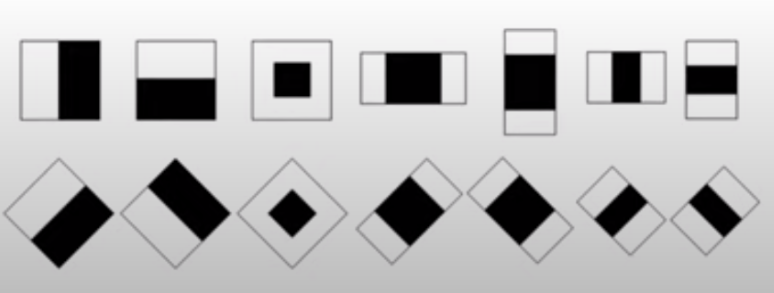
\includegraphics[width=0.4\linewidth]{images/haar_features.png}
  \caption{Haar-Like Features}
\end{figure}

\begin{figure}[htbp]
  \centering
  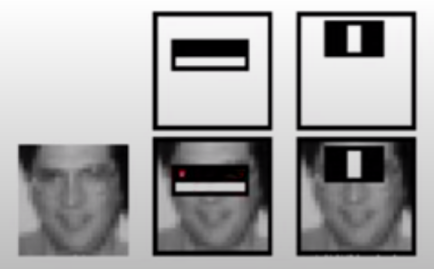
\includegraphics[width=0.4\linewidth]{images/haar_features_1.png}
  \caption{Application of Haar-Like Features}
\end{figure}

\begin{multicols}{2}

\section{Local Binary Pattern Historgrams}
Local Binary Patterns (LBPH) remains a stalwart in face recognition, esteemed for its robustness and adaptability to diverse conditions. This method dissects facial images into local neighborhoods, each representing a distinct region of interest. LBPH examines texture information encoded in pixel intensity values. Its process involves assessing the relationship between the central pixel and its surrounding neighbors, encapsulated within a circular neighborhood. Herein lies LBPH's efficacy: binary encoding of this relationship. For each pixel, LBPH determines whether its intensity surpasses or falls short of its neighbors'. Pixels with higher intensities receive a binary value of 1; otherwise, they receive 0. This binary representation, akin to a digital fingerprint, captures intricate texture details intrinsic to the facial region. By traversing the entire image and repeating this process for every pixel, LBPH assembles a comprehensive mosaic of texture patterns, each encoded into a binary string. These strings, emblematic of the texture variations within each neighborhood, are transformed into decimal values. LBPH distills these values into histograms, encapsulating texture within each neighborhood. Subsequently, these histograms, like miniature texture portraits, are concatenated into a feature vector, representing that of the entire facial image. LBPH transcends limitations of traditional face recognition techniques, surmounting challenges posed by illumination variations, pose changes, and facial expressions (\cite{ahonen2004}; \cite{tan2007}). Thus, LBPH emerges as an efficient method in face recognition, indispensable in applications from security systems to human-computer interaction interfaces.

\end{multicols}

\begin{figure}[htbp]
  \centering
  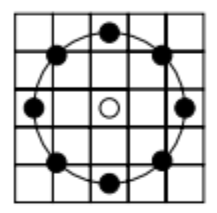
\includegraphics[width=0.4\linewidth]{images/lbph.png}
  \caption{Local Binary Pattern}
\end{figure}

\begin{figure}[htbp]
  \centering
  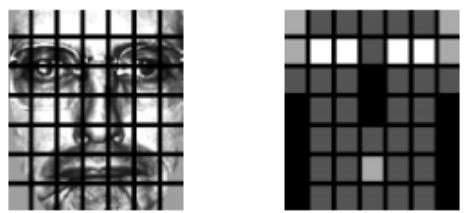
\includegraphics[width=0.4\linewidth]{images/lbph_1.png}
  \caption{LBP Application}
\end{figure}

\begin{figure}[htbp]
  \centering
  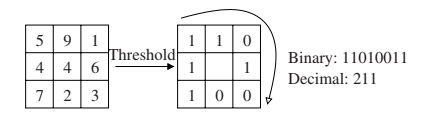
\includegraphics[width=0.4\linewidth]{images/lbph_2.png}
  \caption{Decimal Value Calculation Process}
\end{figure}

\begin{multicols}{2}

\section{PAM Configuraiton Files}
PAM configuration files serve as the cornerstone of user authentication in Linux systems, orchestrating a seamless interaction between applications and authentication mechanisms. At the crux of PAM configuration files lie policy lines, delineating the authentication process for specific applications in great detail. Each policy line comprises several fields, crafted to orchestrate a tailored authentication workflow. The first field, the module type, specifies the category of authentication module to be invoked, ranging from account and session management to the actual authentication logic. Following this, the control flag dictates the behavior of the module, controlling aspects such as whether authentication is required to proceed (required), whether failure should halt the authentication process (requisite), or whether the success of one module should automatically grant access (sufficient). Subsequently, the module path denotes the location of the authentication module's executable file, facilitating its invocation during the authentication process. Parameters, the next field, enable fine-grained customization of module behavior, allowing administrators to specify additional options or configurations. Each parameter is passed to the module upon invocation, influencing its execution and outcome. Through judicious arrangement and configuration of these policy lines, administrators can tailor authentication workflows to meet the security requirements of individual applications, ensuring a fine balance between security and usability. When an application requests authentication, PAM dynamically assembles the configured modules and executes them in the specified order, passing control from one module to the next in a stack-like structure. Each module performs a specific authentication task, such as verifying passwords, checking user permissions, or enforcing multi-factor authentication. By abstracting authentication from application logic, PAM enhances system security and simplifies management, facilitating centralized control over authentication policies across the entire system (\cite{stallings2020}; \cite{love2010}).

\end{multicols}

\begin{figure}[htbp]
  \centering
  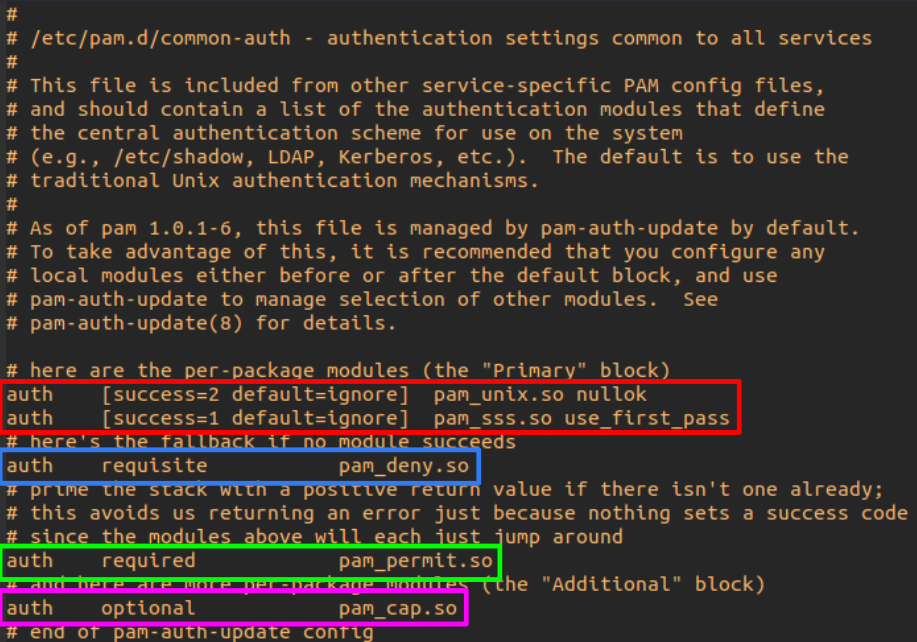
\includegraphics[width=0.4\linewidth]{images/common-auth.png}
  \caption{Module Invocation in `common-auth` PAM Configuration File}
\end{figure}

\begin{multicols}{2}

\section{Face Recognition Development}
The face recognition demo developed in this research exemplifies a robust face recognition system leveraging OpenCV, a powerful computer vision library. At its core, the system integrates two crucial components: a Haar Cascade Classifier for face detection and a Local Binary Patterns Histograms (LBPH) model for face recognition. Firstly, the code initializes the Haar Cascade Classifier by loading a pre-trained model from the specified path \( \text{'CASCADE\_PATH'} \). This classifier detects faces within a video frame by identifying characteristic patterns indicative of facial features. Subsequently, the LBPH model is instantiated using the \( \text{'LBPHFaceRecognizer'} \) class, enabling facial recognition based on texture patterns. The LBPH model is trained with reference faces obtained from the directory specified by \( \text{'REFERENCE\_FACES\_DIR'} \). During training, images are loaded, converted to grayscale, and processed to extract facial features. The LBPH model then learns to associate each face with a corresponding label, facilitating subsequent recognition. Upon model training, the code initializes the camera for real-time face recognition. Each frame captured by the camera undergoes grayscale conversion and histogram equalization to enhance feature contrast. The Haar Cascade Classifier is then employed to detect faces within the frame. Detected faces are passed to the LBPH model for recognition, wherein each face is classified based on its texture pattern. If a match is found with sufficient confidence (determined by \( \text{'MATCH\_THRESHOLD'} \)), the recognized face is marked accordingly. Finally, the code displays the recognition results in real-time, annotating each recognized face with a label and providing information about the total number of faces detected and the number of faces matched. Through this integration of Haar Cascade Classifier and LBPH model, the system achieves robust and efficient face recognition, suitable for diverse applications ranging from security systems to personalized user interfaces (\cite{deng2010}; \cite{ahonen2004}). Below is the source code that facilitates the face recognition demo program utilized for analysis in this integrated research.

\end{multicols}

\begin{adjustwidth}{-1cm}{-1cm}
\begin{verbatim}
#include <opencv2/opencv.hpp>
#include <opencv2/face.hpp>
#include <iostream>
#include <vector>
#include <filesystem> // Add this header for directory_iterator
#include <string>

using namespace cv;
using namespace cv::face;
using namespace std;
namespace fs = std::filesystem;

const string CASCADE_PATH = "/home/henry/Projects/IRC_1/data/haarcascade_frontalface_default.xml";
const string REFERENCE_FACES_DIR = "/home/henry/Projects/IRC_1/data/reference_faces";

const int MATCH_THRESHOLD = 30; // Adjust this value as needed

int main() {
    // Load Haar Cascade Classifier
    CascadeClassifier faceCascade;
    if (!faceCascade.load(CASCADE_PATH)) {
        cerr << "Error loading face cascade.\n";
        return -1;
    }

    // Load LBPH model and train with reference faces
    Ptr<LBPHFaceRecognizer> recognizer = LBPHFaceRecognizer::create();
    vector<Mat> images;
    vector<int> labels;

    // Read reference faces from directory
    try {
        // Load images and labels directly without using read_csv
        for (const auto& entry : fs::directory_iterator(REFERENCE_FACES_DIR)) {
            if (entry.path().extension() == ".png" || entry.path().extension() == ".jpg") {
                Mat img = imread(entry.path().string(), IMREAD_GRAYSCALE);
                images.push_back(img);
                // Get label from filename by parsing
                string filename = entry.path().filename().stem();
                size_t pos = filename.find_last_of("_");
                int label = stoi(filename.substr(pos + 1));
                labels.push_back(label);
            }
        }
        
        // Convert labels to the correct format (CV_32SC1)
        Mat labelsMat(labels.size(), 1, CV_32SC1);
        for (int i = 0; i < labels.size(); ++i) {
            labelsMat.at<int>(i, 0) = labels[i];
        }

        recognizer->train(images, labelsMat);
    } catch (const cv::Exception& e) {
        cerr << "Error training LBPH model: " << e.what() << endl;
        return -1;
    }

    // Open camera
    VideoCapture capture(0);
    if (!capture.isOpened()) {
        cerr << "Error opening camera.\n";
        return -1;
    }

    Mat frame;
    int totalFaces = 0;
    int matchedFaces = 0;
    while (true) {
        capture >> frame;
        if (frame.empty()) {
            cerr << "No frame captured.\n";
            break;
        }

        // Convert frame to grayscale
        Mat grayFrame;
        cvtColor(frame, grayFrame, COLOR_BGR2GRAY);
        equalizeHist(grayFrame, grayFrame);

        // Detect faces using Haar Cascade Classifier
        vector<Rect> faces;
        faceCascade.detectMultiScale(grayFrame, faces);

        totalFaces = faces.size();
        matchedFaces = 0;

        for (const Rect& faceRect : faces) {
            // Extract face region for recognition
            Mat faceROI = grayFrame(faceRect);

            // Perform face recognition
            int label;
            double confidence;
            recognizer->predict(faceROI, label, confidence);

            // Display recognition result
            string labelString = (confidence <= MATCH_THRESHOLD) ? "Match" : "No Match";

            if (confidence <= MATCH_THRESHOLD) {
                matchedFaces++;
            }

            Scalar color = (confidence <= MATCH_THRESHOLD) ? Scalar(0, 255, 0) : Scalar(0, 0, 255);

            // Draw rectangle around the face with matching color
            rectangle(frame, faceRect, color, 2);

            // Display label string
            putText(frame, labelString, Point(faceRect.x, faceRect.y - 5), FONT_HERSHEY_SIMPLEX, 
            0.8, color, 2);
        }

        // Display frame
        string info = "Total Faces: " + to_string(totalFaces) + "   Matched Faces: " 
        + to_string(matchedFaces);
        
        // Draw yellow box behind the text
        int baseline = 0;
        Size textSize = getTextSize(info, FONT_HERSHEY_SIMPLEX, 0.8, 2, &baseline);
        rectangle(frame, Point(5, frame.rows - textSize.height - 10), 
        Point(5 + textSize.width + 10, frame.rows - 5), Scalar(0, 255, 255), FILLED);
        putText(frame, info, Point(10, frame.rows - 10), FONT_HERSHEY_SIMPLEX, 
        0.8, Scalar(255, 0, 255), 2);

        // Show frame
        imshow("Face Recognition", frame);

        // Check for ESC key press
        char c = (char)waitKey(10);
        if (c == 27) {
            break;
        }
    }

    capture.release();
    destroyAllWindows();
    return 0;
}
\end{verbatim}
\end{adjustwidth}

\begin{multicols}{2}

\section{Integration with PAM}
Using the previously mentioned facial recognition logic using OpenCV, the results are integrated with PAM for authentication purposes. Here's a detailed breakdown of how the logic is intricately woven together: The code harnesses OpenCV's powerful face detection and recognition functionalities to execute facial recognition. Initially, it loads a reference image, establishing a foundation for the subsequent training of a LBPH (Local Binary Patterns Histograms) face recognizer. This recognizer is trained with the reference image, laying the groundwork for accurate facial recognition. The authentication process unfolds with a countdown, signaling users to maintain stillness for recording. Following the countdown, the code springs into action, capturing video frames for a defined duration of 5 seconds. With each frame captured, facial recognition is performed diligently, analyzing faces and computing the average confidence level based on recognition outcomes. The integration with PAM is a key aspect of the system, realized through the implementation of PAM authentication functions, each serving a crucial role in the authentication lifecycle. These functions deftly handle user authentication, credential management, and session handling, ensuring a robust authentication mechanism. At the heart of the authentication process lies the authentication function, evaluating the average confidence level obtained from facial recognition. If this confidence level falls below a predetermined threshold, authentication proceeds successfully; otherwise, it fails, safeguarding against unauthorized access. While the PAM library for C++ lacks official documentation, resources such as man pages and online references serve as invaluable guides for leveraging PAM in C and C++ programs. Additionally, the data collection process is orchestrated in great detail, culminating in the calculation of confidence levels of dissimilarity. This crucial step entails assessing how confident the model is that the probe image differs from the trained model with the gallery images. Central to this process is the `performFacialRecognition` function, implementing the same recognition logic demonstrated previously, guaranteeing robust and reliable performance in discerning facial features and computing confidence levels. In essence, this integration of facial recognition with PAM epitomizes the fusion of cutting-edge technology and authentication mechanisms. Through training, integration, and rigorous evaluation, the system stands as a testament to the potential of biometric authentication in bolstering security measures. Below is the structure and implementation of face recognition as a PAM.

\end{multicols}

\begin{adjustwidth}{-1cm}{-1cm}
\begin{verbatim}
#include <security/pam_appl.h>
#include <opencv2/opencv.hpp>
#include <opencv2/face.hpp>
#include <iostream>
#include <vector>
#include <chrono>
#include <thread>

using namespace cv;
using namespace cv::face;
using namespace std;

#define PAM_EXTERN extern "C"

// program settings
const int COUNTDOWN_SECONDS = 5;
const int CONFIDENCE_THRESHOLD = 30;

// function to perform facial recognition and calculate confidence levels
// returns a double for the confidence level
double performFacialRecognition(Mat& frame, Ptr<LBPHFaceRecognizer>& recognizer) {
    CascadeClassifier faceDetector;
    if (!faceDetector.load("/home/henry/Projects/IRC_1/data/haarcascade_frontalface_alt.xml")) {
        cerr << "Error: Could not load face detector." << endl;
        return -1;
    }

    vector<Rect> faces;
    faceDetector.detectMultiScale(frame, faces);

    double totalConfidence = 0.0;
    int recognitionAttempts = 0;

    for (const Rect& face : faces) {
        Mat detectedFace = frame(face);

        int predictedLabel = -1;
        double confidence = 0.0;
        recognizer->predict(detectedFace, predictedLabel, confidence);

        totalConfidence += confidence;
        recognitionAttempts++;
    }

    return recognitionAttempts > 0 ? totalConfidence / recognitionAttempts : -1;
}

// PAM authentication function
PAM_EXTERN int pam_sm_authenticate(pam_handle_t *pamh, int flags, int argc, const char **argv) {
    // loads reference image(s)
    Mat referenceImage = imread("/home/henry/Projects/IRC_1/data/reference_face.jpg", IMREAD_GRAYSCALE);
    if (referenceImage.empty()) {
        cerr << "Error: Could not load reference image." << endl;
        return PAM_AUTH_ERR;
    }

    vector<Mat> referenceImages = { referenceImage };

    // creates LBPH recognizer and trains with reference image(s)
    Ptr<LBPHFaceRecognizer> recognizer = LBPHFaceRecognizer::create();
    recognizer->train(referenceImages, vector<int>(referenceImages.size(), 0));

    // opens the camera and catches any hardware exceptions
    VideoCapture cap(0);
    if (!cap.isOpened()) {
        cerr << "Error: Could not open camera." << endl;
        return PAM_AUTH_ERR;
    }

    // counts down and notifies the user to hold still for recording
    for (int i = COUNTDOWN_SECONDS; i > 0; i--) {
        cout << "Please hold still. Recording will begin in " << i << " seconds." << endl;
        std::this_thread::sleep_for(chrono::seconds(1));
    }

    // records for 5 seconds and collects confidence levels
    auto start = chrono::steady_clock::now();
    int frameCount = 0;
    double totalConfidence = 0.0;

    while (chrono::steady_clock::now() - start < chrono::seconds(5)) {
        Mat frame;
        cap >> frame;

        if (frame.empty()) {
            cerr << "Error: Failed to capture frame." << endl;
            return PAM_AUTH_ERR;
        }

        // converts the frame to grayscale for image analysis
        Mat grayFrame;
        cvtColor(frame, grayFrame, COLOR_BGR2GRAY);

        // performs facial recognition on the frame
        double confidence = performFacialRecognition(grayFrame, recognizer);
        if (confidence < 0) {
            cerr << "Error: Facial recognition failed." << endl;
            return PAM_AUTH_ERR;
        }

        totalConfidence += confidence;
        frameCount++;
    }

    // calculates the average confidence
    double averageConfidence = totalConfidence / frameCount;
    cout << "Average confidence: " << averageConfidence << endl;

    // authenticates the user based on the average confidence level
    if (averageConfidence < CONFIDENCE_THRESHOLD) {
        printf("SUCCESS!\n");
        return PAM_SUCCESS; 
    } else {
        printf("FAILURE\n");
        return PAM_AUTH_ERR; 
    }
}

// PAM function for setting credentials 
PAM_EXTERN int pam_sm_setcred(pam_handle_t *pamh, int flags, int argc, const char **argv) {
    return PAM_SUCCESS; 
}

// PAM function for opening the session
PAM_EXTERN int pam_sm_open_session(pam_handle_t *pamh, int flags, int argc, const char **argv) {
    return PAM_SUCCESS;
}

// PAM fucntion for closing/cleaning up the session
PAM_EXTERN int pam_sm_close_session(pam_handle_t *pamh, int flags, int argc, const char **argv) {
    return PAM_SUCCESS;
}
\end{verbatim}
\end{adjustwidth}

\begin{multicols}{2}

\section{Custom PAM Invocations}
First, as a proof-of-concept demonstration , a custom bypass module was developed to showcase the low-level function of a properly configured PAM. A module was developed using the same PAM library that with logic that simply returned a success to the PAM mechanism. This module was simply pushed onto the stack of module invocations in the `su` PAM configuration file. After attempting to switch to another user, a success was returned to the mechanism, granting  automatic access. This process can be seen below.

\end{multicols}

\begin{figure}[htbp]
  \centering
  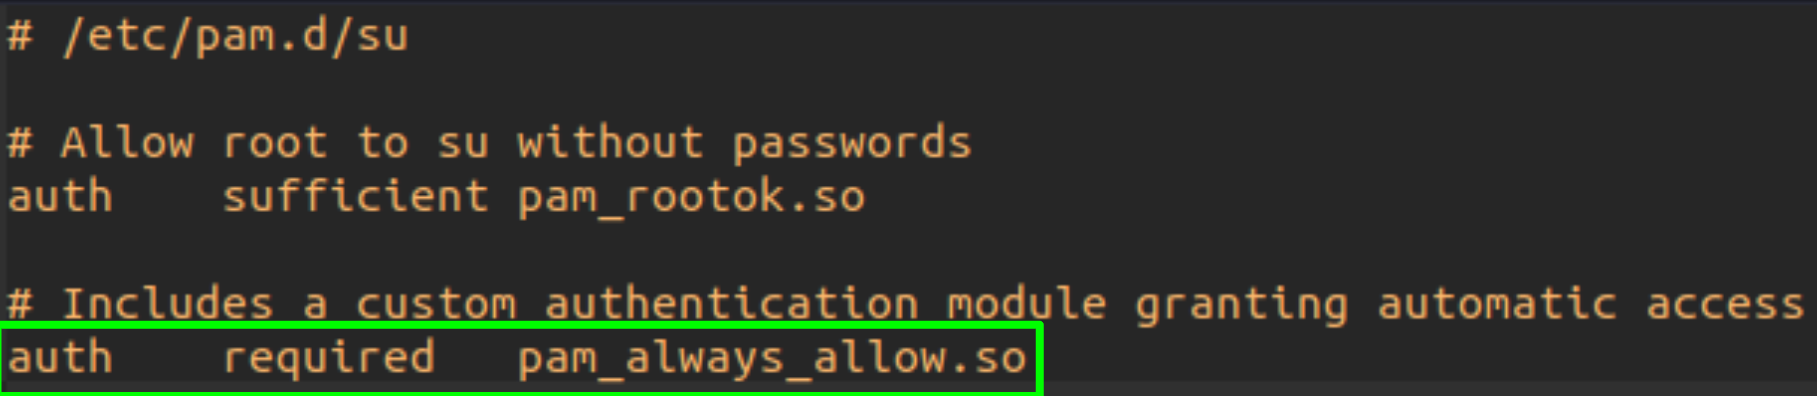
\includegraphics[width=0.4\linewidth]{images/bypass_config.png}
  \caption{Bypass Module in `su` PAM Configuration File}
\end{figure}

\begin{figure}[htbp]
  \centering
  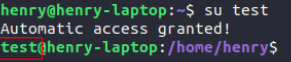
\includegraphics[width=0.4\linewidth]{images/bypass_implementation.png}
  \caption{Implementation of Bypass Module}
\end{figure}

\begin{multicols}{2}

\section{Results and Evaluation}
During the integration of facial recognition logic with PAM for authentication, functional facial recognition logic faced runtime errors when utilizing the camera for video frame capture. Although the facial recognition itself worked correctly, successfully detecting and recognizing faces in the captured frames, the runtime errors hindered the PAM authentication process. These errors, likely due to hardware-related issues, prevented the PAM mechanism from authorizing authentication. To address this, an alternative debugging approach was adopted. Instead of real-time video capture, a separate program utilized pre-captured images as probe images for facial recognition. This approach isolated hardware-related issues, allowing focused testing of the facial recognition algorithm and its integration with PAM. With this modified setup, facial recognition successfully operated without encountering runtime errors, providing insights into system performance and reliability. 

\end{multicols}

\begin{figure}[htbp]
  \centering
  \begin{subfigure}[b]{0.3\textwidth}
    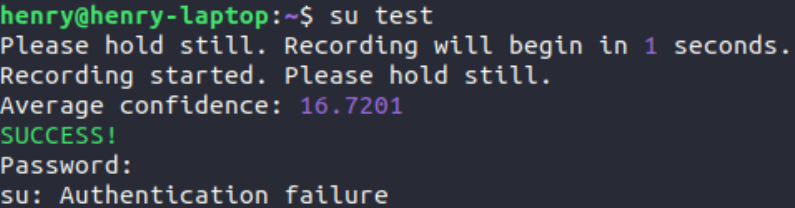
\includegraphics[width=\textwidth]{images/runtime_error.png}
    \caption{Runtime Error in Module}
  \end{subfigure}
  \hfill
  \begin{subfigure}[b]{0.3\textwidth}
    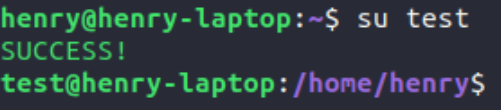
\includegraphics[width=\textwidth]{images/runtime_debug.png}
    \caption{Runtime Debugging Output}
  \end{subfigure}
  \hfill
  \begin{subfigure}[b]{0.3\textwidth}
    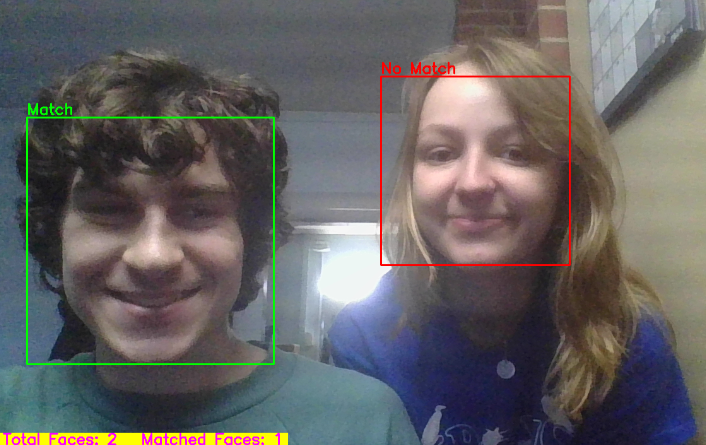
\includegraphics[width=\textwidth]{images/demo_result.png}
    \caption{Successful Real-Time Detection and Recognition of A Matching Face Against A Non-Match}
  \end{subfigure}
  \caption{Face Recognition Results}
\end{figure}

\begin{multicols}{2}

\section{Conclusion and Future Work}
In summary, this project has made significant strides in integrating facial recognition technology with PAM for authentication, despite encountering runtime errors during real-time detection, likely due to hardware limitations. Debugging efforts, including the use of a separate program for image probing, identified and resolved issues, ensuring successful module functionality. Although the models exhibited moderate accuracy, further training with expanded datasets could enhance performance. The integration of facial recognition with PAM showcases its potential in bolstering security measures, particularly in access control systems. Leveraging technologies like OpenCV and PAM, this project sets the stage for future developments in biometric authentication, offering scalable and reliable solutions for security challenges. Looking ahead, areas for further improvement include refining models for better accuracy and exploring integration with additional security methods.

\end{multicols}

\bibliographystyle{apalike}
\bibliography{irc_1_ref.bib}

\end{document}
